% this comment scales down all text equally
\documentclass[8pt]{beamer}
\usetheme{Boadilla} % Required for inserting images
\usepackage{caption}

%additional packages that can be removed ----
%\setbeamertemplate{conjecture}[numbered]
% \newtheorem{conjecture}[theorem]{Conjecture}
% \setbeamertemplate{SLT Claims}[numbered]


% Add this before \begin{document}
% automatically create section slides
\AtBeginSection[]
{
  \begin{frame}
  \frametitle{}
  \centering
  \huge{\insertsectionhead}
  \end{frame}
}

% --------------------------------------------

\title{Breaking Down R1}
\subtitle{Reasoning Via Reinforcement Learning}
\author[]{Zach Liu}
\institute{CAISH}
\date{Feb 2025}

\begin{document}

\begin{frame}
\titlepage
\end{frame}

\begin{frame}{Contents}
    \tableofcontents
\end{frame}

\section{Preliminaries}

\subsection{Transformers}

\begin{frame}{Autoregressive Models}

\centering
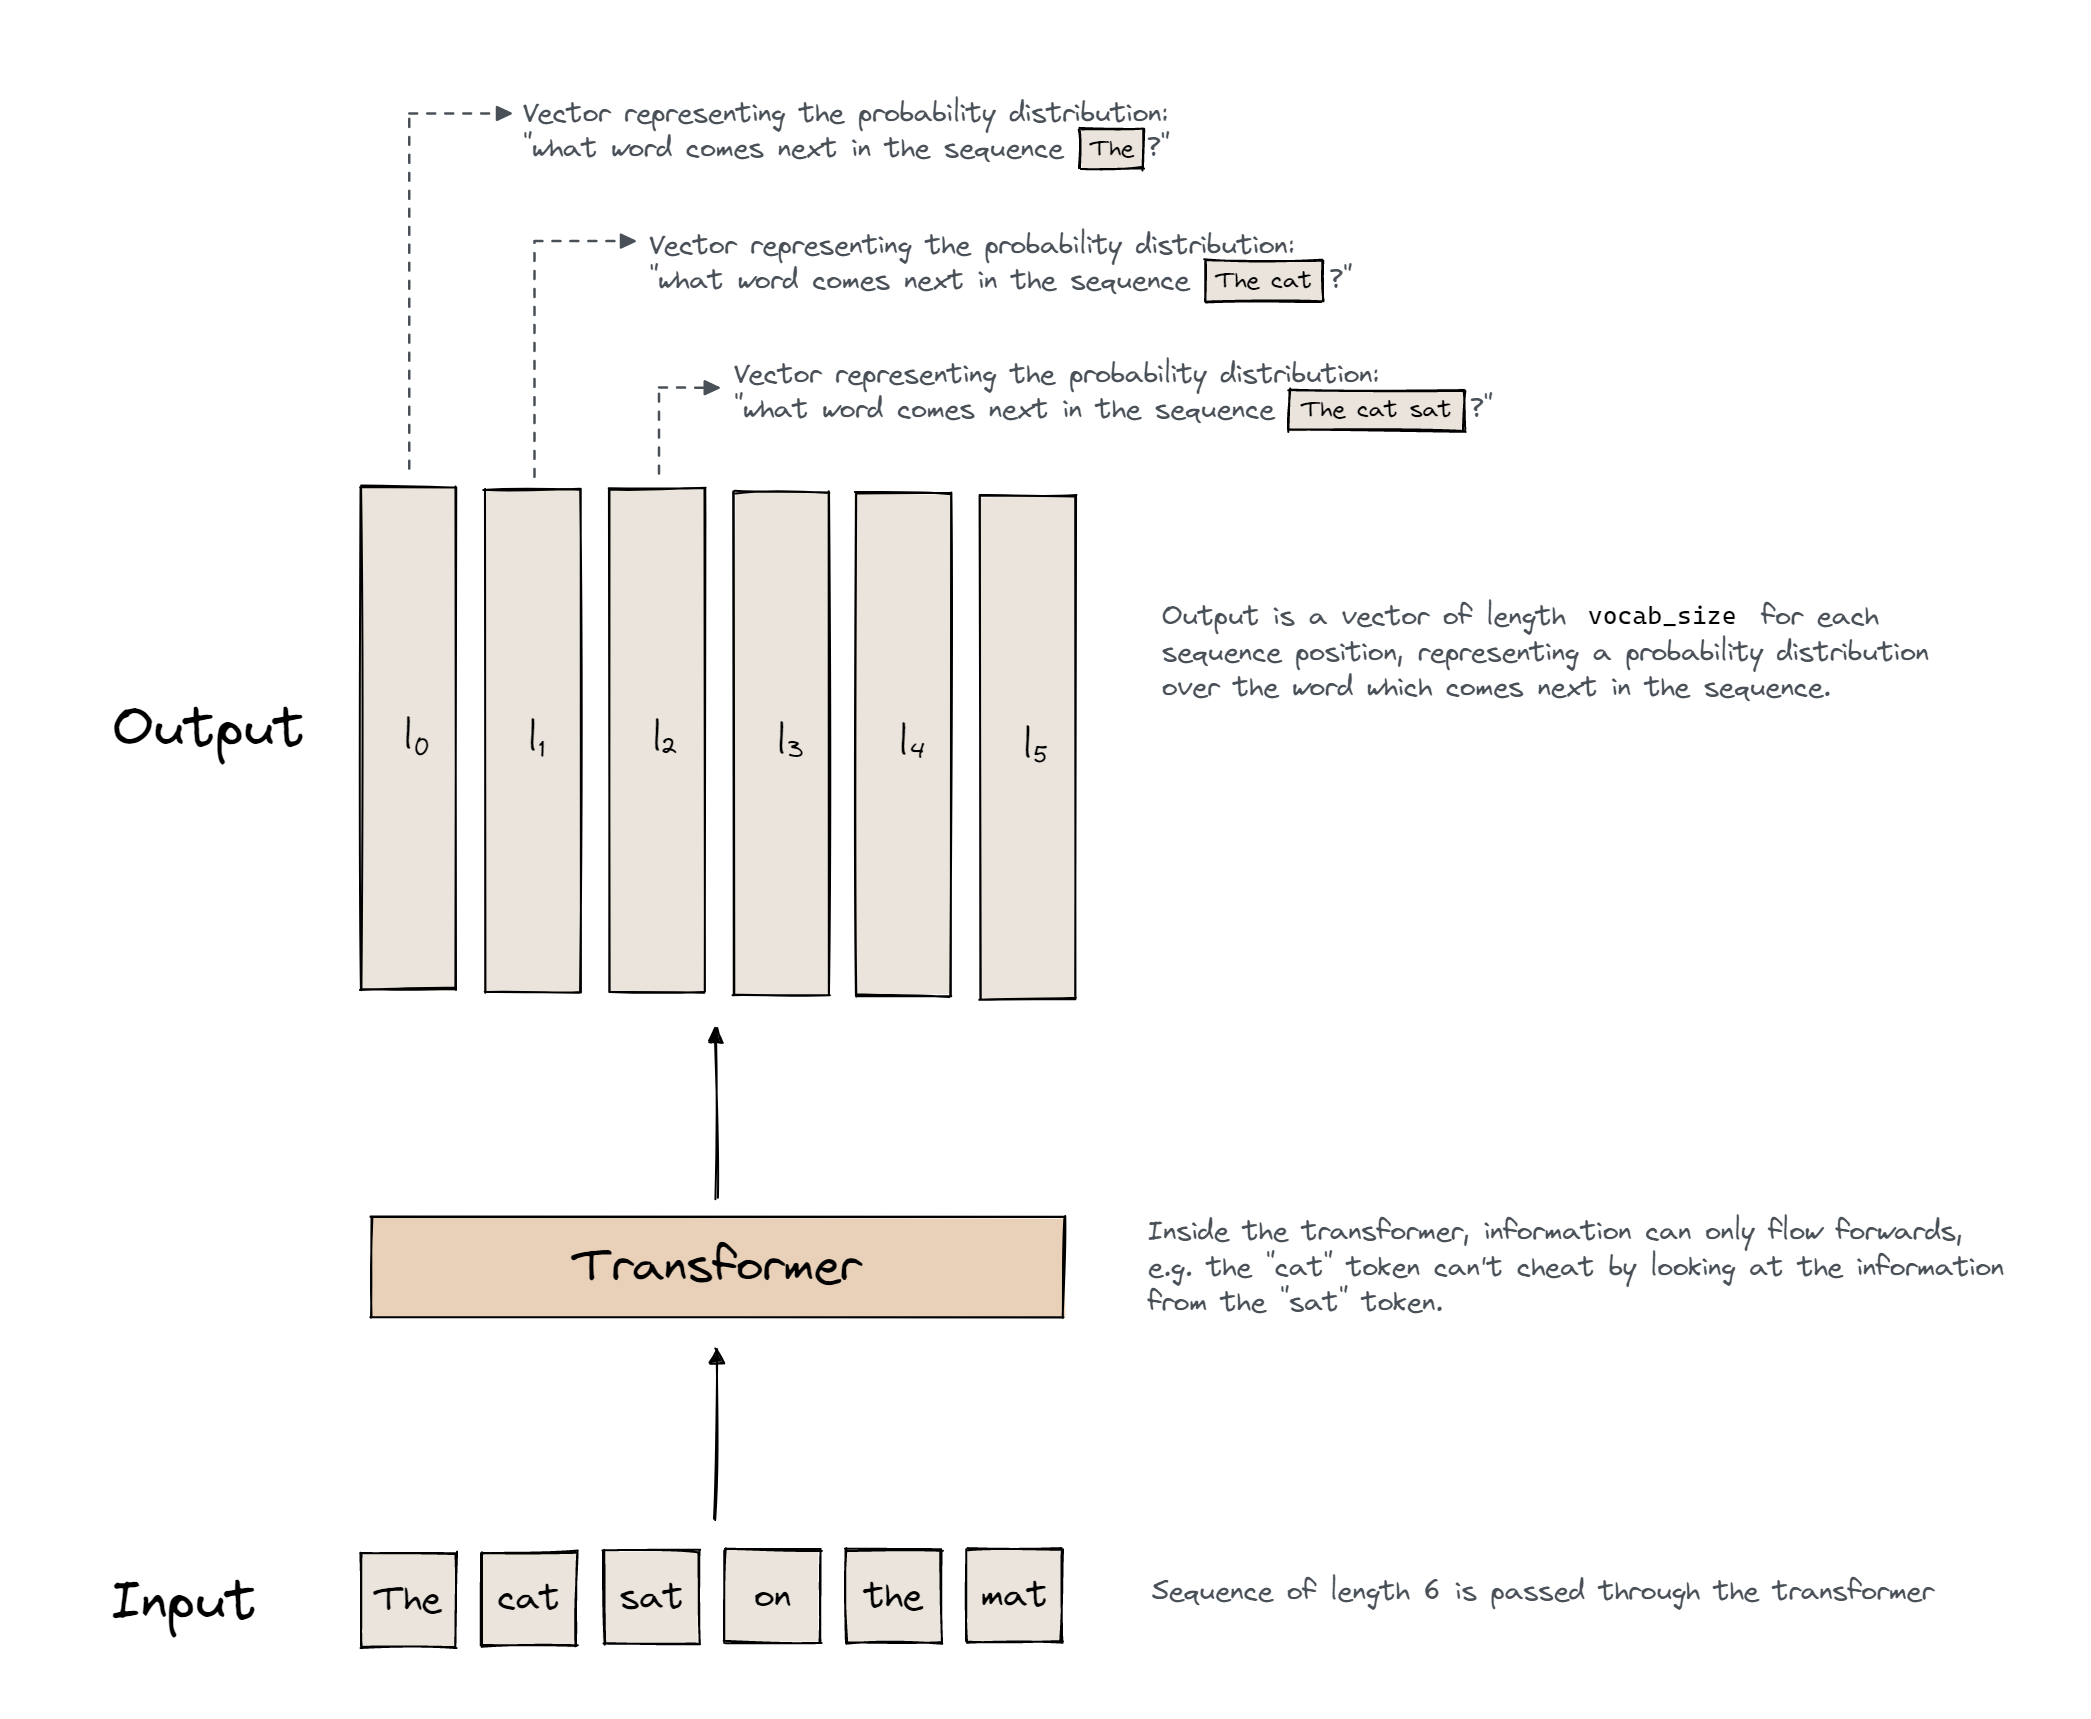
\includegraphics[width=0.7\textwidth]{figures/transformer-overview.png}

{\small
\begin{equation}
p(x_1,\ldots,x_N) = \prod_{n=1}^N p(x_n|x_1,\ldots,x_{n-1})
\end{equation}
}
\end{frame}

\begin{frame}{Transformer Architecture}
\centering
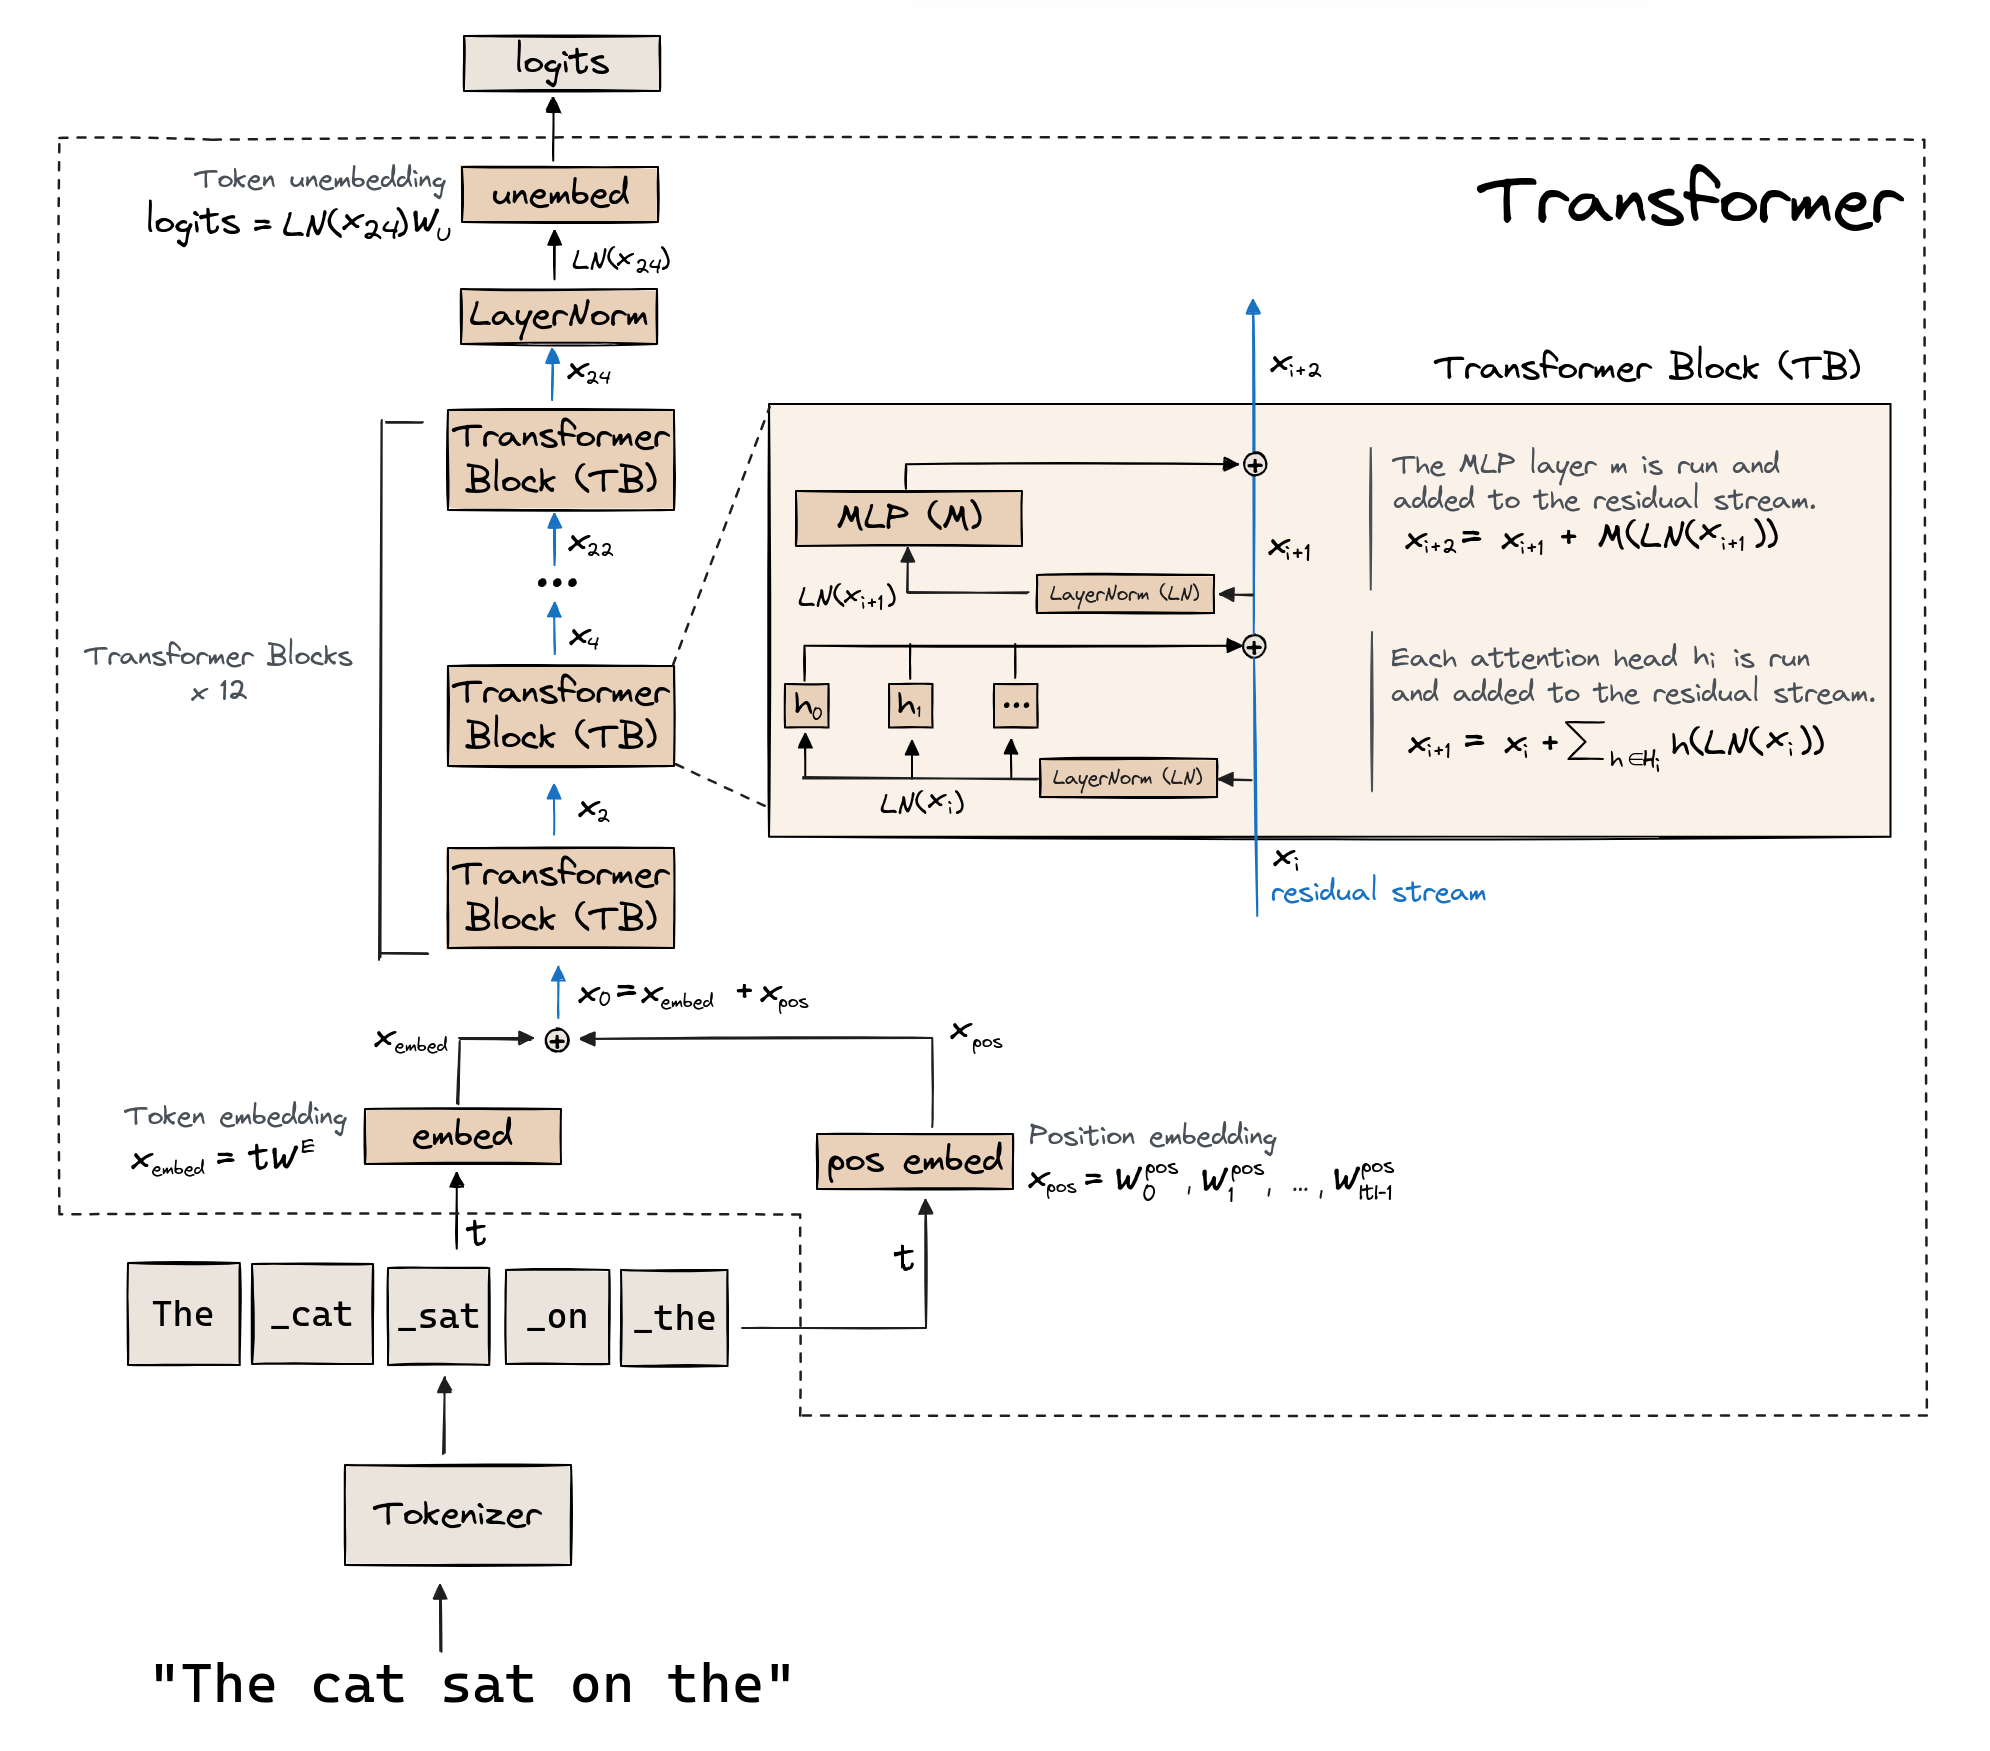
\includegraphics[width=0.8\textwidth]{figures/transformer-arch.png}
\end{frame}

\subsection{Reinforcement Learning}

\begin{frame}{Reinforcement Learning Setup}
\begin{itemize}
    \item The agent in \textbf{state} $s$ issues an \textbf{action} $a$ to the environment, and the environment replies with \textbf{state, reward} pairs $(s',r)$. We can define a trajectory $\tau$ as a sequence of states and actions: $s_0, a_0, r_1, a_1, r_2, s_2, a_2, r_3...$
    \item The agent chooses actions using a policy $\pi$ which can either be a deterministic function $a=\pi(s)$ from states to actions, or more generally actions are sampled $a \sim \pi(\cdot|s)$
    \item The \textbf{return} at time $t$ is the sum of rewards obtained \textit{after} time $t$ until the time $T$ when the terminal state is reached, discounted by how far into the future:

    \begin{equation}
        G_t = \sum_{k=0}^{\infty} \gamma^k r_{t+k+1} = r_{t+1} + \gamma r_{t+2} + \gamma^2 r_{t+3} ...
    \end{equation}

\end{itemize}
\end{frame}

\begin{frame}{Value Functions and Advantages}

\begin{itemize}

    \item The \textbf{state value function} $V_\pi(s)$ is the expected return, if you start in state $s$ and always act according to policy $\pi$:

    \begin{equation}
    V_{\pi}(s) = \mathbb{E}_{\pi}\left[G_t| s_t = s\right]
    \end{equation}

    \item The \textbf{action value function} is the expected return if you start in state $s$, take an arbitrary action $a$ (which may not have come from the policy), and then afterwards forever act according to policy $\pi$:
    \begin{equation}
    Q_\pi(s, a) = \mathbb{E}_{\pi} \left[G_t| s_t = s, a_t = a\right]
    \end{equation}

    \item The \textbf{advantage function} describes how much better it is to take a specific action $a$ in state $s$, over randomly selecting an action according to $\pi(\cdot|s)$, assuming you act according to $\pi$ forever after:

    \begin{equation}
    A_\pi(s, a) = Q_\pi(s, a) - V_\pi(s)
    \end{equation}

\end{itemize}
    
\end{frame}

\begin{frame}{Trust Region Policy Optimization (TRPO)}

Let $\pi_\theta$ denote a policy with parameters $\theta$. We aim to maximize the expected return $J$ of policy $\pi_\theta$, where we take expectation over all possible trajectories $\tau$ generated by following policy $\pi_\theta$

$$J(\pi_\theta) = \underset{\tau \sim \pi_\theta}{\mathbb{E}}[G(\tau)]$$

To achieve the optimum $\pi_\theta$ that maximizes J, we can iteratively update $\pi_\theta_k$ according to:

\begin{equation*}
\theta_{k+1} = \arg \max_\theta \mathcal{L}(\theta_k, \theta) = \arg \max_\theta \underset{s,a\sim\pi_{\theta_k}}{\mathbb{E}} \left[L(s, a, \theta_k, \theta)\right], \quad \text{s.t. } \bar{D}_{KL}(\theta\|\theta_k) \leq \delta
\end{equation*}

where $\mathcal{L}(\theta_k, \theta)$ is the \textit{surrogate advantage}, a measure of how policy $\pi_\theta$ performs relative to the old policy $\pi_{\theta_k}$ using data from the old policy:

\begin{equation*}
L(s, a, \theta_k, \theta) = \frac{\pi_\theta(a|s)}{\pi_{\theta_k}(a|s)} A_{\pi_{\theta_k}}(s,a)
\end{equation*}

TRPO updates policies by taking the largest step possible to improve performance, while satisfying a special constraint on how close the new and old policies are allowed to be.
\end{frame}

\begin{frame}{Proximal Policy Optimization (PPO)}
Proximal Policy Optimization updates policies via:

\begin{equation*}
\theta_{k+1} = \arg \max_\theta \mathcal{L}(\theta_k, \theta) = \arg \max_\theta \underset{s,a\sim\pi_{\theta_k}}{\mathbb{E}} \left[L(s, a, \theta_k, \theta)\right],
\end{equation*}

typically taking multiple steps of SGD to maximize the objective. Here $L$ is given by:

\begin{equation}
    L(s, a, \theta_k, \theta) = \min\Bigg(\frac{\pi_\theta(a|s)}{\pi_{\theta_k}(a|s)}A_{\pi_{\theta_k}}(s,a), \text{clip}\left(\frac{\pi_\theta(a|s)}{\pi_{\theta_k}(a|s)}, 1-\epsilon, 1+\epsilon\right)A_{\pi_{\theta_k}}(s,a)\Bigg)
\end{equation}

\vspace{1em}

PPO-Clip doesn’t have a KL-divergence term in the objective and doesn’t have a constraint at all. Instead relies on specialized clipping in the objective function to remove incentives for the new policy to get far from the old policy.

\end{frame}

\begin{frame}{Advantage Estimation in PPO}
    \textbf{Generalized Advantage Estimation (GAE)} is used in PPO to estimate the advantage function:
    
    \begin{equation}
    A_t = \sum_{l=0}^{\infty} (\gamma \lambda)^l \delta_{t+l}
    \end{equation}

    where:
    %make this item separation smaller
    \begin{itemize}\setlength{\itemsep}{5pt}
        \item $\delta_t = r_t + \gamma V(s_{t+1}) - V(s_t)$ (TD error)
        \begin{itemize}
            \item the reward $r_t$ is usually given by a trained (neural) reward model
        \end{itemize}
        \item $\gamma$ is the discount factor
        \item $\lambda$ is the GAE parameter (tradeoff between bias and variance)
        \item $V(s)$ is the value function estimate, from value network
        \begin{itemize}
            \item Often a value network $V_\psi$ needs to
be trained alongside the policy model $\pi_\theta$ to estimate the value, often as big as the policy model itself
        \end{itemize}
    \end{itemize}

    \vspace{1em}

    \textbf{Advantage Calculation in PPO:}
    
    The truncated form for practical implementation:
    
    \begin{equation}
    A_t = \delta_t + (\gamma \lambda) \delta_{t+1} + (\gamma \lambda)^2 \delta_{t+2} + \dots
    \end{equation}
    
\end{frame}

\begin{frame}{General RL Training Setup}
\small
    % Define the overall RL objective: maximize the expected return.
    \textbf{Objective:}
    \[
    J(\pi_\theta) = \mathbb{E}_{\tau \sim \pi_\theta}\left[\sum_{t=0}^{T} \gamma^t r_t\right],
    \]
    where \(\tau = \{s_0, a_0, r_1, s_1, a_1, \dots, s_T\}\) is a trajectory. For LLMs, \textit{actions} $a_t$ here are \textit{tokens}!
    
    \vspace{0.8em}
    
    % Policy gradient theorem provides the gradient direction for updating the policy.
    \textbf{Policy Gradient:}
    \[
    \nabla_\theta J(\pi_\theta) = \mathbb{E}_{s,a \sim \pi_\theta}\left[\nabla_\theta \log \pi_\theta(a|s) \, Q^{\pi_\theta}(s,a)\right],
    \]
    or equivalently, using the advantage function \(A^{\pi_\theta}(s,a)\):
    \[
    \nabla_\theta J(\pi_\theta) = \mathbb{E}_{s,a \sim \pi_\theta}\left[\nabla_\theta \log \pi_\theta(a|s) \, A^{\pi_\theta}(s,a)\right].
    \]
    
    \vspace{0.8em}
    
    % Trajectories are collected by running the current policy in the environment.
    \textbf{Trajectory Collection:}  
    LLM interacts with the environment (reward model) to sample trajectories. For each timestep:
    \[
    s_t \xrightarrow{\pi_\theta} a_t \rightarrow r_{t+1},\, s_{t+1}.
    \]
    
    \vspace{0.8em}
    
    % Returns and advantages are computed to estimate the quality of actions.
    \textbf{Return and Advantage Calculation:}
    \[
    G_t = \sum_{k=0}^{\infty} \gamma^k r_{t+k+1}, \quad
    A(s_t,a_t) = Q^{\pi_\theta}(s_t,a_t) - V^{\pi_\theta}(s_t).
    \]
    Generalized Advantage Estimation (GAE) are used to compute \(A(s_t,a_t)\) practically
    
    \vspace{0.8em}
    
    % Finally, update the policy parameters by moving in the direction of the estimated gradient.
    \textbf{Policy Update:}
    \[
    \theta_{k+1} = \theta_k + \alpha\, \nabla_\theta J(\pi_\theta),
    \]
    Using the computed advantages, update the policy parameters and value network by maximizing a surrogate objective (e.g., the PPO objective) to favor actions with higher expected returns. Repeat until agent’s performance converges.
\end{frame}


\section{R1-Zero}

\begin{frame}{Group Relative Policy Optimization (GRPO)}
\centering
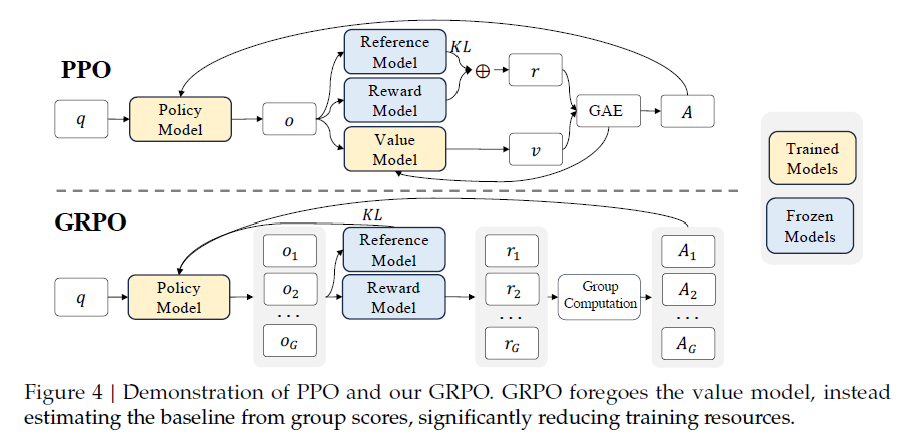
\includegraphics[width=0.9\textwidth]{figures/grpo.png}
\end{frame}

\begin{frame}{GRPO}

DeepSeek uses GRPO, created in-house, which foregoes the value network and estimates the advantages directly from group rewards instead.

\vspace{1em}

For each question $q$, GRPO samples a group of outputs $\{o_i\}_{i=1}^G$ from the old policy $\pi_{\theta_{\text{old}}}$ and then optimizes the policy model $\pi_\theta$ by maximizing:

\begin{align*}
\mathcal{J}_{\text{GRPO}}(\theta) &= \mathbb{E}[q \sim P(Q), \{o_i\}_{i=1}^G \sim \pi_{\theta_{\text{old}}}(Q|q)] \\
&\quad \cdot \frac{1}{G}\sum_{i=1}^G\left(\min\left(\frac{\pi_\theta(o_i|q)}{\pi_{\theta_{\text{old}}}(o_i|q)}A_i, \text{clip}\left(\frac{\pi_\theta(o_i|q)}{\pi_{\theta_{\text{old}}}(o_i|q)}, 1-\epsilon, 1+\epsilon\right)A_i\right) - \beta\mathbb{D}_{KL}(\pi_\theta\|\pi_{\text{ref}})\right), \tag{1}
\end{align*}

\begin{equation*}
\mathbb{D}_{KL}(\pi_\theta\|\pi_{\text{ref}}) = \frac{\pi_{\text{ref}}(o_i|q)}{\pi_\theta(o_i|q)} - \log\frac{\pi_{\text{ref}}(o_i|q)}{\pi_\theta(o_i|q)} - 1, \tag{2}
\end{equation*}

where $\epsilon$ and $\beta$ are hyper-parameters, and $A_i$ is the advantage \footnote{Instead of adding KL
penalty in the reward like in PPO, GRPO regularizes by directly adding the KL divergence between the
trained policy and the reference policy to the loss, avoiding complicating the calculation of advantage $A$}
\end{frame}

\begin{frame}{GRPO Advantages}
Advantages $A_i$ are computed using group rewards $\{r_1,r_2,\ldots,r_G\}$:

\begin{equation*}
A_i = \frac{r_i - \text{mean}(\{r_1,r_2,\ldots,r_G\})}{\text{std}(\{r_1,r_2,\ldots,r_G\})} \tag{3}
\end{equation*}

\vspace{1em}

As the value network is typically another model of comparable size as
the policy model, it brings a substantial memory and computational burden. GRPO eliminates value network completely! 
\end{frame}

\begin{frame}{Reward Modelling}

R1-Zero uses a rule-based reward system consisting of:

\begin{itemize}\setlength{\itemsep}{8pt}
\item \textbf{Accuracy rewards:} The accuracy reward model evaluates whether the response is correct.
    \begin{itemize}\setlength{\itemsep}{3pt}
        \item For math problems with deterministic results, can easily check if right or wrong. Provider higher reward if right.
        \item For LeetCode problems, a compiler can be used to generate feedback based on predefined test cases
    \end{itemize}

\item \textbf{Format rewards:} Enforces the model to put its thinking process between \texttt{<think>} and \texttt{</think>} tags.
\end{itemize}

\vspace{1em}
Usually for LLMs, a neural reward model (neural network used to estimate rewards) is used to provide rewards, as human preferences or requirements are difficult to define in a rules-based way. However, R1 does not use any neural reward model:
\begin{itemize}
    \item Neural reward model may suffer from reward hacking
    \item Retraining the reward model needs additional training resources and it complicates the whole training pipeline
\end{itemize}

\end{frame}

\begin{frame}{Performance}
\centering
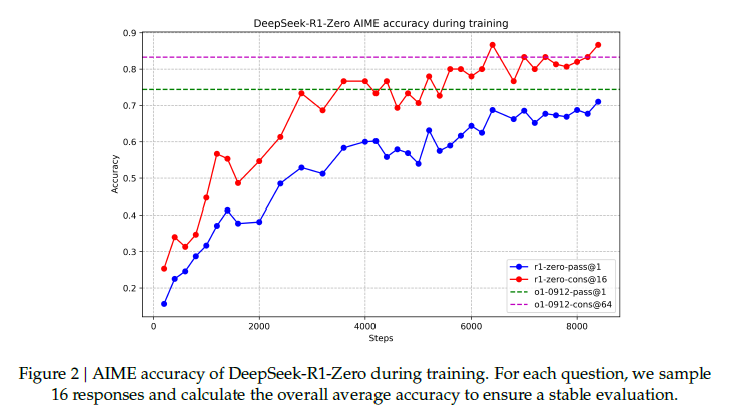
\includegraphics[width=0.8\textwidth]{figures/aime.png}

\begin{itemize}
    \item No Supervised-Fine-Tuning involved in R1-Zero
    \item Majority voting bring performance on AIME benchmark from 71\% to 86\%
\end{itemize}

\end{frame}

\begin{frame}{Self-Evolution}
\centering
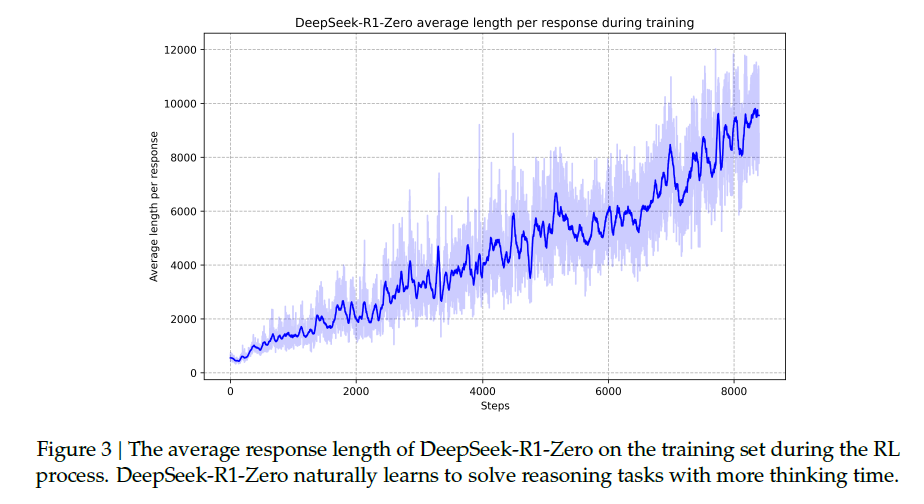
\includegraphics[width=0.8\textwidth]{figures/perf.png}

\begin{itemize}
    \item R1-Zero naturally acquires the
ability to solve increasingly complex reasoning tasks by leveraging extended test-time computation (increased Chain-Of-Thought)
    \item Behaviours like backtracking and reflection emerge
\end{itemize}

\end{frame}

\begin{frame}{Problems}

\begin{itemize}
    \item Poor Readability of Chain-Of-Thought
    \item Language Mixing
\end{itemize}

\vspace{1em}

Probably some form of reward over-optimization, more efficient to reason in its own language and achieve higher reward

\end{frame}

\section{R1 Training Pipeline}

\subsection{Phase 1: Cold Start}

\begin{frame}{Phase 1: Cold Start}
\centering
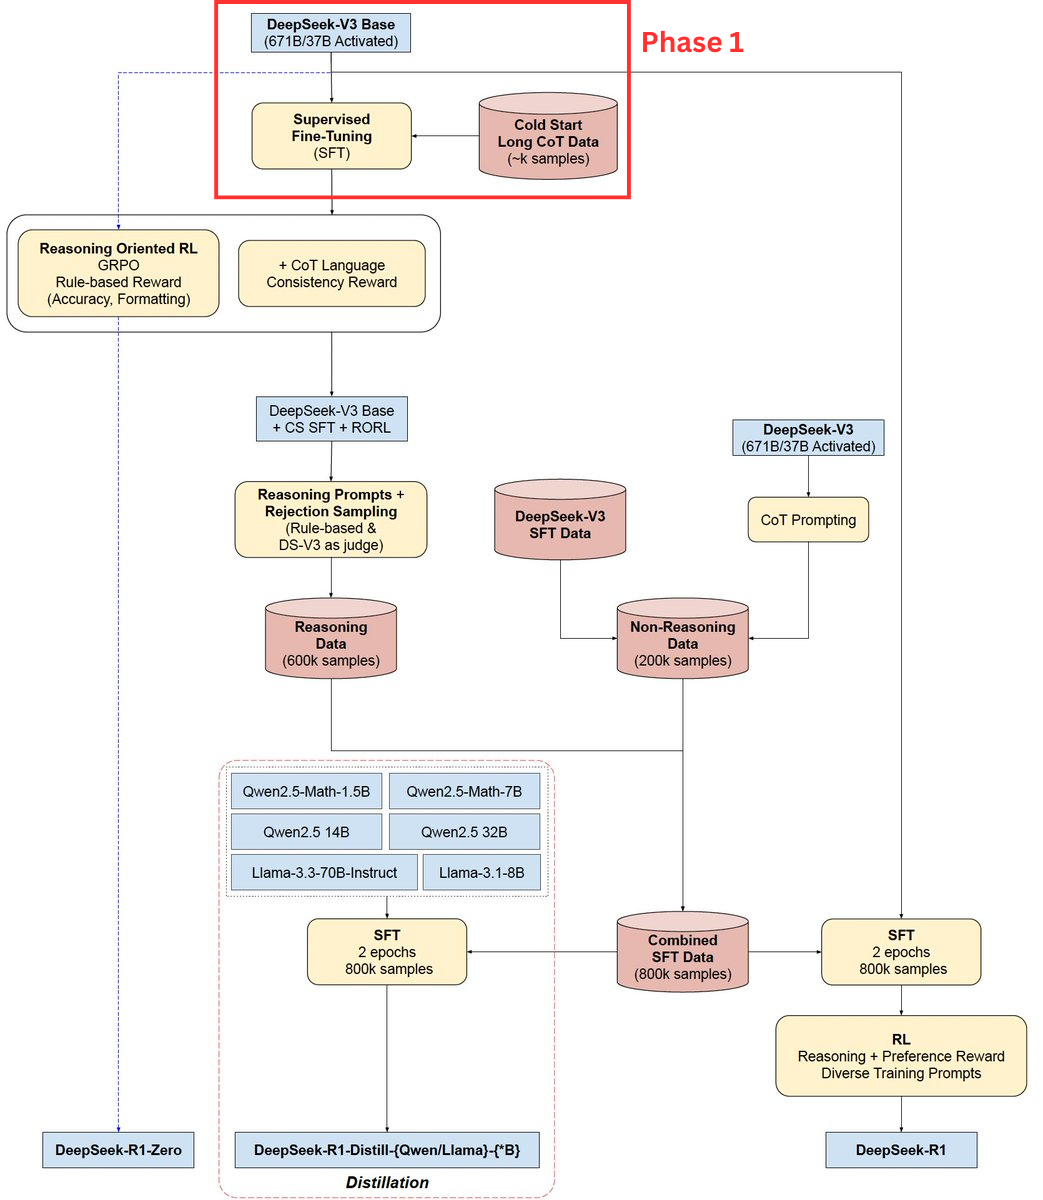
\includegraphics[width=0.6\textwidth]{figures/phase1.png}
\end{frame}

\begin{frame}{Phase 1: Cold Start}

\begin{itemize} \setlength{\itemsep}{10pt}
\item Construct and collect small amounts (thousands) of long CoT data to fine-tune V3
    \begin{itemize} \setlength{\itemsep}{5pt}
    \item Using few-shot prompting on V3 with long CoT examples
    \item Direct prompting on V3 for detailed answers with reflection
    \item Gathering DeepSeek-R1-Zero outputs with human post-processing
    \end{itemize}

\item Key advantages:
    \begin{itemize} \setlength{\itemsep}{5pt}
    \item \textbf{Readability:} R1-Zero has unreadable responses. We define output format as \texttt{|special\_token|<reasoning\_process>|special\_token|<summary>} so reasoning process (CoT) and summary of reasoning provided
    \item \textbf{Potential:} Carefully designed patterns with human priors show better performance vs R1-Zero
    \end{itemize}
\end{itemize}
    
\end{frame}
\subsection{Phase 2: Reasoning Reinforcement Learning}

\begin{frame}{Phase 2: Reasoning Reinforcement Learning}
\centering
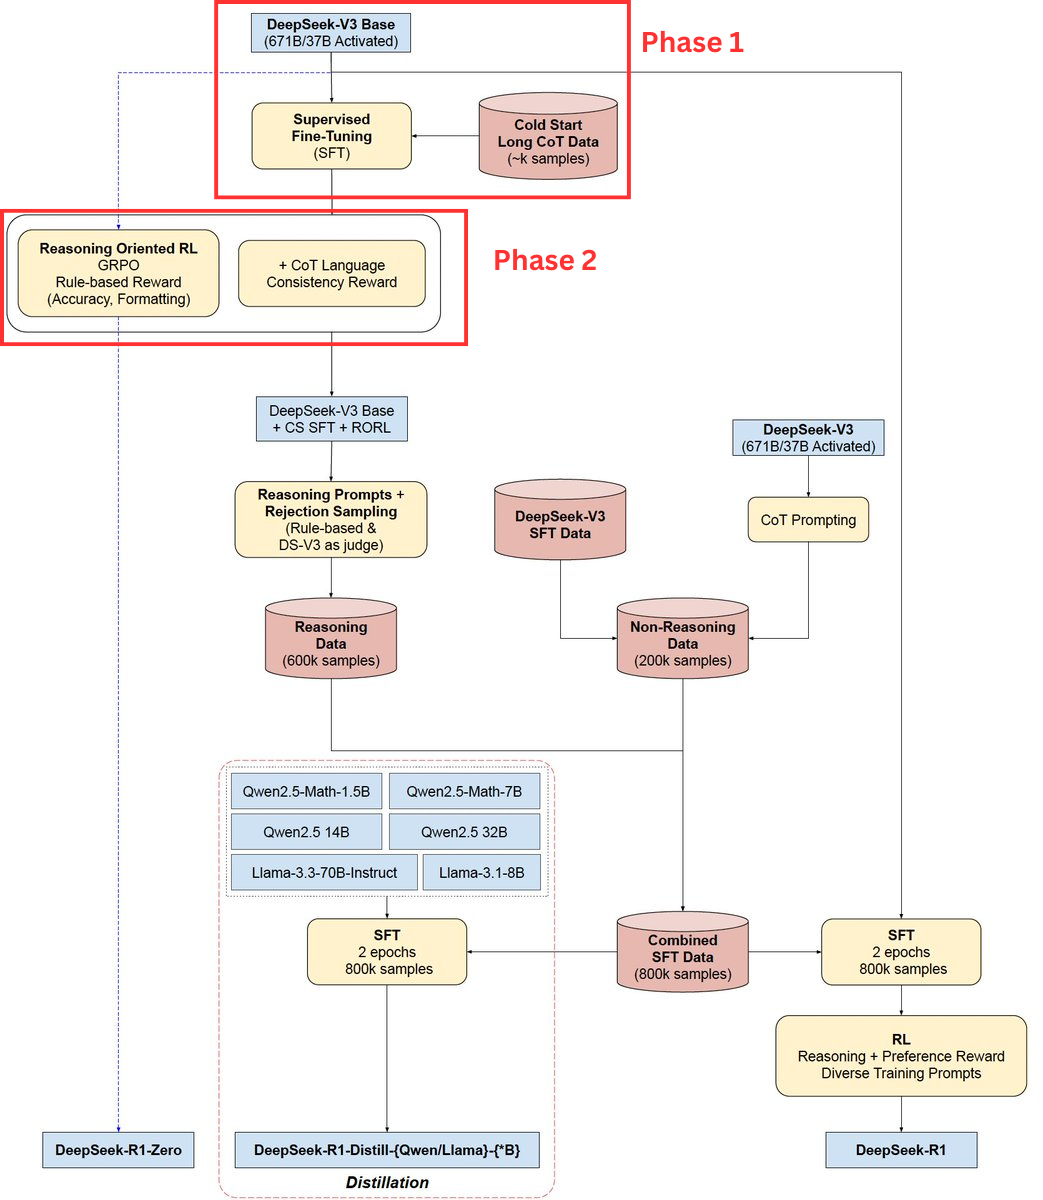
\includegraphics[width=0.6\textwidth]{figures/phase2.png}
\end{frame}

\begin{frame}{Phase 2: Reasoning Reinforcement Learning}
After cold start fine-tuning, apply large-scale RL training similar to DeepSeek-R1-Zero:

\begin{itemize}\setlength{\itemsep}{10pt}
    \item Focus on reasoning-intensive tasks:
        \begin{itemize}
        \item Coding, mathematics, science, logic reasoning
        \item Well-defined problems with clear solutions
        \end{itemize}
    
    \item Language Consistency:
        \begin{itemize}
        \item CoT exhibits language mixing in multi-language prompts
        \item Introduce language consistency reward, measured as proportion of target language words in CoT
        \end{itemize}

\end{itemize}

\vspace{1em}

Final reward function combines reasoning task accuracy, language consistency reward, and formatting reward to train until convergence.
\end{frame}

\subsection{Phase 3: Rejection Sampling and Supervised Fine-Tuning}

\begin{frame}{Phase 3: Rejection Sampling and Supervised Fine-Tuning}
\centering
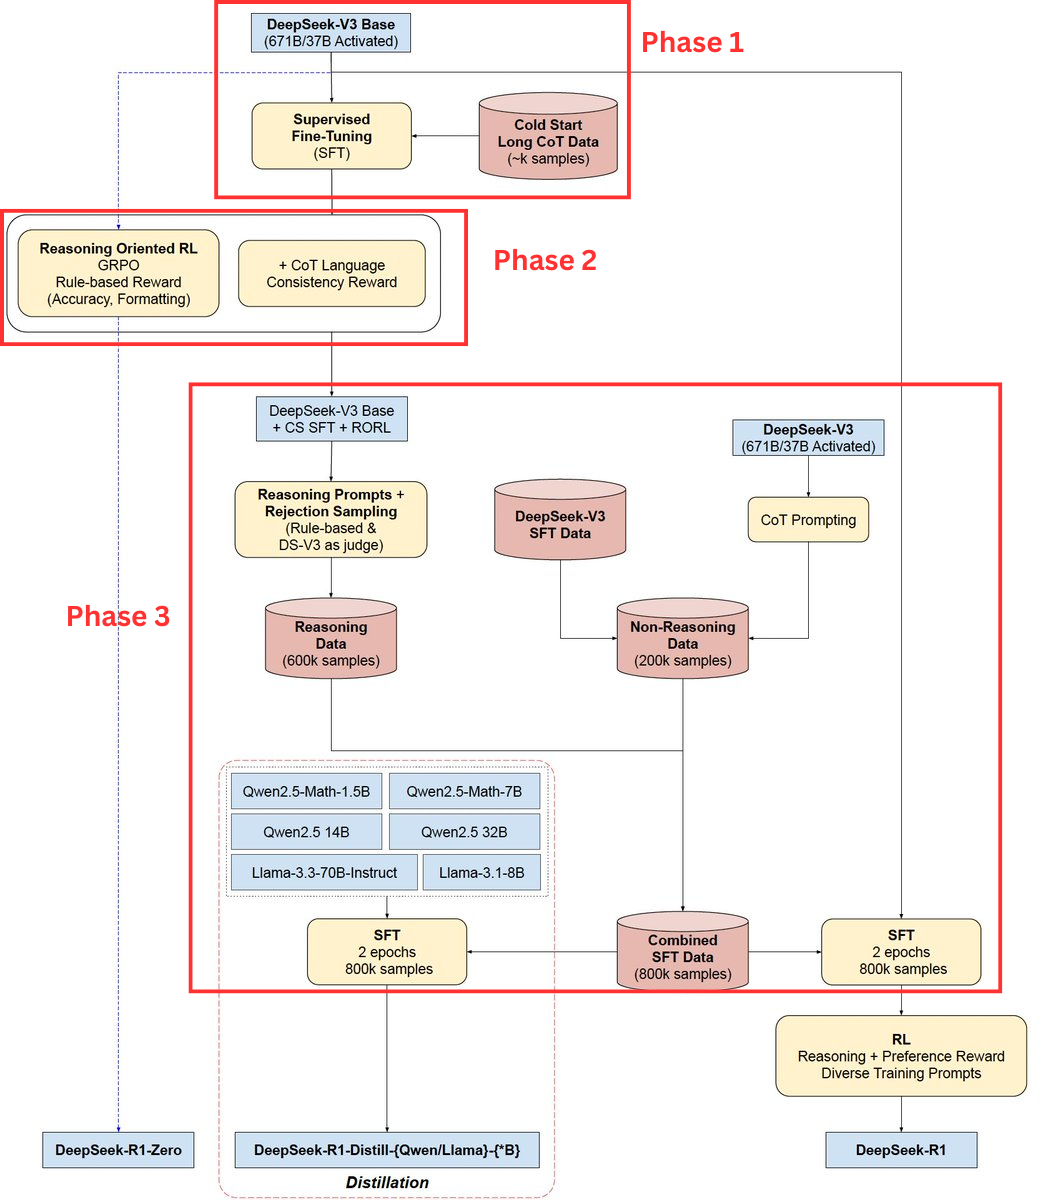
\includegraphics[width=0.6\textwidth]{figures/phase3.png}
\end{frame}

\begin{frame}{Phase 3: Rejection Sampling and Supervised Fine-Tuning}

After RL convergence, collect SFT data from checkpoint for further training. Include

\vspace{1em}

\begin{columns}[t]
\begin{column}{0.5\textwidth}
\textbf{Reasoning Data (600k samples)}
\begin{itemize}
\item Rejection sampling from RL checkpoint
\item Expanded dataset includes:
    \begin{itemize}
    \item Rule-based rewards
    \item Generative rewards via DeepSeek-V3 as LLM-Judge
    \end{itemize}
\item Quality filters:
    \begin{itemize}
    \item Remove mixed languages
    \item Filter long paragraphs
    \item Remove chaotic code blocks
    \end{itemize}
\end{itemize}
\end{column}

\begin{column}{0.5\textwidth}
\textbf{Non-Reasoning Data (200k samples)}
\begin{itemize}
\item Types:
    \begin{itemize}
    \item Writing
    \item Factual QA
    \item Self-cognition
    \item Translation
    \end{itemize}
\item Reuse SFT data for DeepSeek-V3
\end{itemize}
\end{column}
\end{columns}

\vspace{1em}
Final fine-tuning on \textbf{DeepSeek-V3-Base}: 2 epochs on combined 800k samples
\end{frame}

\subsection{Phase 4: Diverse Reinforcement Learning Phase}

\begin{frame}{Phase 4: Diverse Reinforcement Learning Phase}
\centering
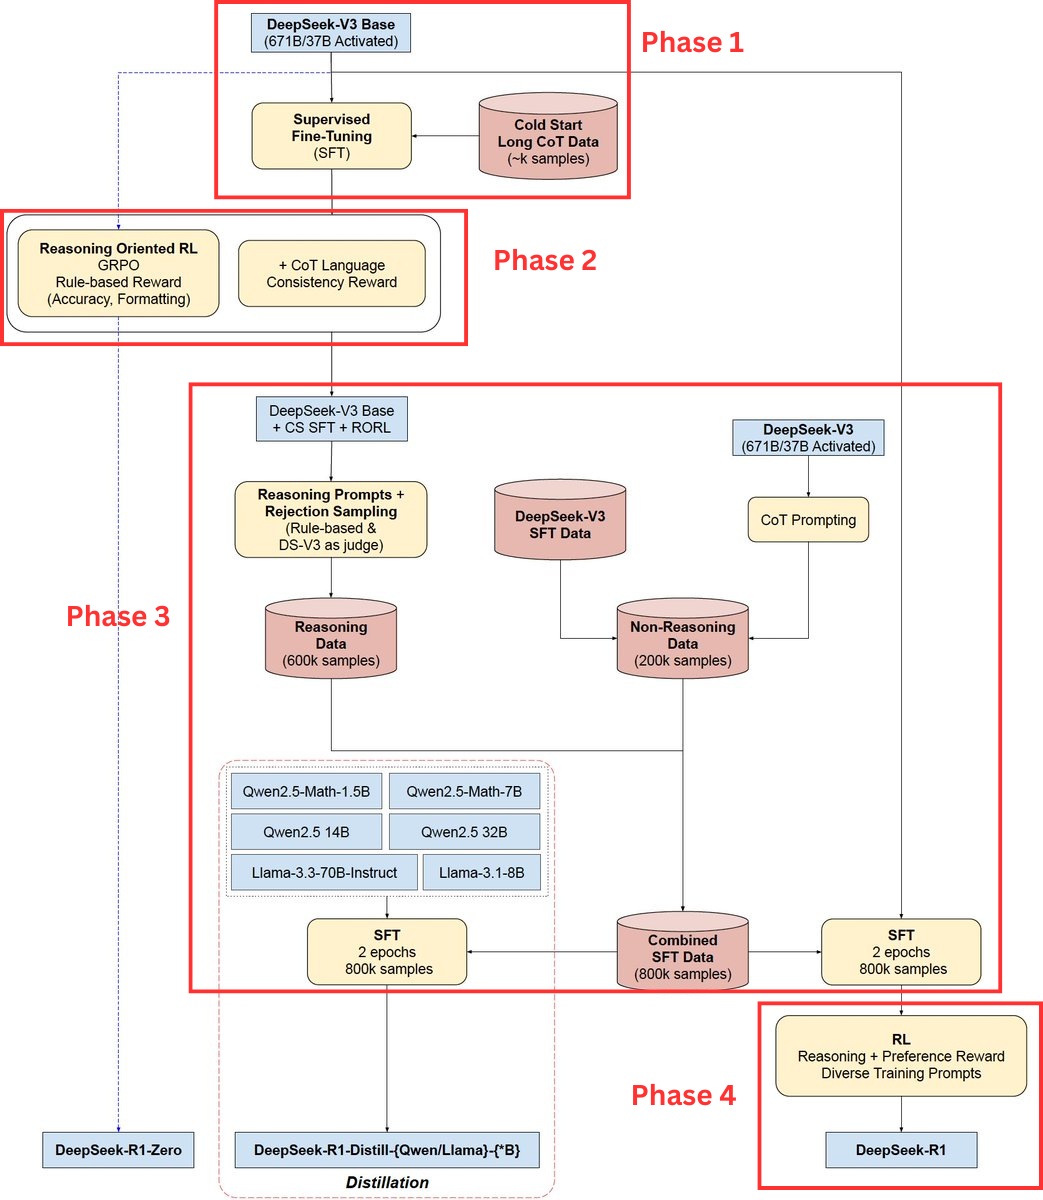
\includegraphics[width=0.6\textwidth]{figures/phase4.png}
\end{frame}

\begin{frame}{Phase 4: Diverse Reinforcement Learning Phase}

Secondary RL stage to align with human preferences while improving, helpfulnes, harmlessness, and reasoning:

\vspace{1em}

\begin{columns}[t]
\begin{column}{0.5\textwidth}
\textbf{Training Approach}
\begin{itemize}
\item Reasoning data:
    \begin{itemize}
    \item Same approach as DeepSeek-R1-Zero
    \item Rule-based rewards on Math, code, logical reasoning
    \end{itemize}
\item General data:
    \begin{itemize}
    \item Reward model as in DeepSeek V3
    \item Use preference pairs
    \end{itemize}
\end{itemize}
\end{column}

\begin{column}{0.5\textwidth}
\textbf{HHH Criteria}
\begin{itemize}
\item Helpfulness:
    \begin{itemize}
    \item Focus on final summary in summary tag is useful and relevance
    \item Preserves reasoning process in the reasoning tag
    \end{itemize}
\item Harmlessness:
    \begin{itemize}
    \item Evaluate full response for potential biases or hamful content
    \end{itemize}
\end{itemize}
\end{column}
\end{columns}

\end{frame}

\section{R1 Engineering Unlocks}

\begin{frame}{Engineering Unlocks}

Insane software and hardware optimizations

\begin{itemize} \setlength{\itemsep}{8pt}
    \item Multi-Head Latent Attention (for efficient inference)
        \begin{itemize}
            \item Low-rank join compression for \textbf{K,Q,V} matrices to reduce key-value cache memory usage
        \end{itemize}
    \item DeepSeekMoE with Auxiliary-Loss-Free Load Balancing (efficient training)
    \begin{itemize}
        \item 671B parameters, but only which 37B are activated for each token
    \end{itemize}

    \item Multi-Token Prediction Objective
    
\end{itemize}
    
\end{frame}

\end{document}
